
\documentclass[fancyheadings, fancychapter, sureport]{Classes/a-report}
\ifpdf
    \hypersetup{
    	backref,
        colorlinks  = true,
        pdftitle    = Modelo de documentação,
        pdfauthor   = {Marco Reis, marco.a.reis@gmail.com},
        pdfsubject  = Mestre em Engenharia,
        pdfcreator  = Subtitulo,
        pdfproducer = PDFLatex,
        pdfkeywords = {documentação, latex, dissertação, tese}}
 \fi
\usepackage[utf8]{inputenc}
\usepackage[brazil]{babel}
\usepackage{longtable}
\usepackage{dcolumn}
\usepackage{multirow}
\usepackage{lscape}
\usepackage{rotating}
\usepackage{cite}
\usepackage[left=3cm,top=3cm,right=2cm,bottom=2cm]{geometry}
\usepackage[alf]{abntex2cite}
\usepackage{ifpdf}
\usepackage{shadow}
\usepackage{wrapfig}
\usepackage[normalem]{ulem}
\usepackage{makeidx}
\usepackage{yfonts}
\usepackage{algorithm}
\usepackage{algorithmic}
\usepackage{lmodern}
\usepackage[T1]{fontenc}
\usepackage{indentfirst}
\usepackage{color}
\usepackage{microtype}
\usepackage{lipsum}
\usepackage{caption}
\usepackage{subcaption}
\usepackage{plantuml}
\makeindex 
\setlength{\LTcapwidth}{\textwidth}

\newtheorem{theorem}{Teorema}
\newtheorem{definition}[theorem]{Definição}

\renewcommand{\backrefpagesname}{Citado na(s) página(s):~}
% Texto padrão antes do número das páginas
\renewcommand{\backref}{}
% Define os textos da citação
\renewcommand*{\backrefalt}[4]{
	\ifcase #1 %
		Nenhuma citação no texto.%
	\or
		Citado na página #2.%
	\else
		Citado #1 vezes nas páginas #2.%
	\fi
}
% 
% -------------------------------------------------------------------------------
% Início do documento raiz
\begin{document}
% Definição do título da página
    \university{Universidade Positivo}
	%\faculty{Programa de...}
	%\school{Escola de...}
% 
    %\course{Engenharia Elétrica}
    \typework{Relatório Final}
% 
	%\course{Mestrado em Modelagem Computacional e Tecnologia Industrial}
	%\typework{Disserta\c{c}\~ao de mestrado}
	%\typework{Exame de Qualificação de Mestrado}
% 
	%\course{Engenharia Elétrica}
	%\typework{Tese de doutorado}
	%\typework{Exame de Qualificação de doutorado}
%
% -------------------------------------------------------------------------------
% Informações gerais
    \thesistitle{Análise e Projeto de Sistemas - Aplicação prática e teorica}
    \hidevolume
    \thesisvolume{Volume 1 of 1}
    \thesisauthor{ANA PAULA DA SILVA RGM: 35652209}
    \thesisauthorr{GIOVANNI VENÇÃO RGM: 041761693}
    \thesisauthorrr{GUSTAVO C. DE ALMEIDA RGM: 36800457}
    \thesisauthorrrr{JOÃO M. STACOVIAKI RGM: 42043719}
    \thesisauthorrrrr{MARIANNE C. BUENO RGM: 41984269}
    \thesisauthorrrrrr{SABRINA DE S. BORGES RGM: 42018897}
    \thesisadvisor{Prof. Marco Reis, M.Eng.}
    %\hidecoadvisor
    %\thesiscoadvisor{Marco Reis}
    \thesismonthyear{Abril de 2025}
% 
    \maketitlepage
%
% ----------------------------------------------------------------------------
% Inserir Folha de rosto, Nota de estilo, folha de assinaturas, dedicatoria
    \begin{folharosto}

\begin{center}
\theauthor \\
\theauthorr \\
\theauthorrr \\
\theauthorrrr \\
\theauthorrrrr \\
\theauthorrrrrr \\

\end{center}
\ \\
\ \\
\ \\
\ \\
\ \\
\begin{spacing}{2}
   \begin{center}
   {\LARGE {\bf \thetitle}}
   \end{center}
\end{spacing}
\ \\
\ \\
\ \\
\vspace*{85mm}
% \begin{flushright}

%    \begin{list}{}{
%       \setlength{\leftmargin}{7.5cm}
%       \setlength{\rightmargin}{0cm}
%       \setlength{\labelwidth}{0pt}
%       \setlength{\labelsep}{\leftmargin}}

%       \item \thetypework apresentada ao \thefaculty, Curso de \thecourse
%       do \theuniversity, como requisito parcial para a obten\c{c}\~ao do
%       t\'itulo de {\bf \thedegreetitle}.

%       \begin{list}{}{
%       \setlength{\leftmargin}{0cm}
%       \setlength{\rightmargin}{0cm}
%       \setlength{\labelwidth}{0pt}
%       \setlength{\labelsep}{\leftmargin}}

%       \item \'Area de conhecimento: Interdisciplinar

%       \item Orientador: \theadvisor
%       \newline \hspace*{2.1cm}  %{\it \theuniversity}

%       \end{list}
%    \end{list}

% \end{flushright}
\ \\
\ \\
\ \\
\ \\
%\begin{spacing}{1.5}
   \begin{center}
   Curitiba \par
   \theuniversity \par
   2025
   \end{center}
%\end{spacing}

\end{folharosto}

    %\begin{notaestilo}
Esta \thetypeworkthree foi elaborada considerando as normas de
estilo (i.e. est\'eticas e estruturais) propostas aprovadas pelo
colegiado do \thefacultytwo e est\~ao dispon\'iveis em formato
eletr\^onico ({\it download} na P\'agina Web
http:$//$ead.fieb.org.br$/$portal\_faculdades$/$dissertacoes-e-teses-mcti.html
ou solicita\c{c}\~ao via e-mail \`a secretaria do
programa) e em formato impresso somente para consulta. \\

Ressalta-se que o formato proposto considera diversos itens das
normas da Associa\c{c}\~ao Brasileira de Normas T\'ecnicas (ABNT),
entretanto opta-se, em alguns aspectos, seguir um estilo pr\'oprio
elaborado e amadurecido pelos professores do programa de
p\'os-gradua\c{c}\~ao supracitado.

\end{notaestilo}

    %\begin{folhaassinaturas}

%\thispagestyle{empty}

\def\signature#1#2{\parbox[b]{1in}{\smash{#1}\vskip12pt}
\hfill \parbox[t]{3in}{\shortstack{\vrule width 3in height
0.4pt\\\small#2}}}

\def\InstituicaoMembro#1#2{\parbox[b]{1in}{\smash{#1}\vskip12pt}
\hfill \parbox[t]{3in}{\shortstack{\vrule width 3in \\\small#2}}}

\def\signaturepage{%

    \begin{spacing}{1.5}
        \begin{center}
        {\LARGE \theuniversity} \\
        {\large \thefaculty} \\
        {\large \thecourse} \\
        \end{center}
    \end{spacing}

   \vskip 0.25in plus 0.4in minus 0.1in

    \begin{spacing}{1.5}
        \begin{sloppypar}
        A Banca Examinadora, constitu\'ida pelos professores abaixo
        listados, leram e recomendam a aprova\c{c}\~ao [com distin\c{c}\~ao] da
        \thetypeworktwo, intitulada ``\thetitle",
        apresentada no dia (dia) de (m\^es) de (ano), como requisito
        parcial para a obten\c{c}\~ao do t\'itulo de {\bf \thedegreetitle}.\\
        \end{sloppypar}
    \end{spacing}

    \def\sigskip{\vskip0.15in plus 0.2in minus 0.1in}
    \def\beginskip{\vskip0.3875in plus 0.2in minus 0.1in}

    \beginskip
    \signature{Orientador:}{Prof. Dr. \theadvisor} \\
    \InstituicaoMembro{}{\theuniversity} \\

    \sigskip
    \beginskip
    \signature{Membro externo da Banca:}{Prof. Dr. Nome completo} \\
    \InstituicaoMembro{}{Institui\c{c}\~ao do membro da banca} \\

    \sigskip
    \beginskip
    \signature{Membro externo da Banca:}{Prof. Dr. Nome completo} \\
    \InstituicaoMembro{}{Institui\c{c}\~ao do membro da banca} \\

    %\sigskip
    %\beginskip
   % \signature{Membro interno da Banca:}{Prof. Dr. Nome completo} \\
   % \InstituicaoMembro{}{Institui��o do membro da banca} \\

    \vfill
    \newpage
    \setcounter{page}{3}
}
%*********************************************************************


\signaturepage


\end{folhaassinaturas}

    %\include{Others/dedicatoria}
    %\include{Others/agradecimentos}
%
% ----------------------------------------------------------------------------
% Resumo/abstract, sumário e siglas
    \begin{romanpagenumbers}
        \begin{thesisresumo}
Este relatório apresenta o desenvolvimento de um projeto prático da disciplina de Análise e Projeto de Sistemas, cujo objetivo foi criar um site portfólio personalizado para um cliente real. A pesquisa foi conduzida com base em uma abordagem mista, combinando elementos do modelo Waterfall com práticas do framework Scrum, permitindo maior controle e flexibilidade durante o desenvolvimento. Inicialmente, foram levantados os requisitos do cliente por meio de reuniões e formulários, e posteriormente elaborados os diagramas UML (casos de uso, sequência e classes), definição da arquitetura da solução, modelagem dos processos e escolha das tecnologias (HTML, CSS, JavaScript e GitHub Pages). O projeto permitiu a aplicação prática dos conceitos estudados, além do desenvolvimento de habilidades interpessoais. Como contribuição, o trabalho entrega não apenas um produto funcional e esteticamente alinhado às preferências do cliente, mas também um exemplo de documentação completa para projetos de software, reforçando a importância da engenharia de requisitos e da validação contínua junto ao cliente.

\ \\

% use de três a cinco palavras-chave

\textbf{Palavras-chave}: Análise de Sistemas, Projeto de Sistemas, Portfólio Web, Desenvolvimento Front-end, Requisitos de Software.

\end{thesisresumo}

        \begin{thesisabastract}
This report presents the development of a practical project for the Systems Analysis and Design course, aimed at creating a personalized portfolio website for a real client. The research was conducted using a hybrid approach, combining elements of the Waterfall model with practices from the Scrum framework, enabling greater control and flexibility throughout development. Initially, client requirements were gathered through meetings and forms, followed by the creation of UML diagrams (use cases, sequence, and class), definition of the solution architecture, process modeling, and selection of technologies (HTML, CSS, JavaScript, and GitHub Pages). The project enabled the practical application of course concepts, as well as the development of interpersonal skills. As a contribution, the work delivers not only a functional product aligned with the client's aesthetic preferences but also a complete example of software project documentation, reinforcing the importance of requirements engineering and continuous client validation. 

\ \\

% use de tr�s a cinco palavras-chave

\textbf{Keywords}: Systems Analysis, Systems Design, Web Portfolio, Front-End Development, Software Requirements.

\end{thesisabastract}

        % Make list of contents, tables and figures
        \thesiscontents
        \newpage
        %Include other required section
        %\begin{thesisabbreviations}
\begin{footnotesize}
\begin{longtable}[l]{p{2cm}l}
  tprax   \dotfill & \thefaculty \\
  WWW       \dotfill &  World Wide Web \\
\end{longtable}
\end{footnotesize}
\end{thesisabbreviations}

        %\begin{thesissymbols}
\begin{footnotesize}
\begin{longtable}[l]{p{2cm}l}
  $\partial$   \dotfill  & Bla bla bla \\
  $\prod$       \dotfill & ble ble ble \\
  $\partial$   \dotfill  & Bla bla bla \\
  $\prod$       \dotfill & ble ble ble \\
  $\partial$   \dotfill  & Bla bla bla \\
  $\prod$       \dotfill & ble ble ble \\
  $\partial$   \dotfill  & Bla bla bla \\
  $\prod$       \dotfill & ble ble ble \\
  $\partial$   \dotfill  & Bla bla bla \\
  $\prod$       \dotfill & ble ble ble \\
  $\partial$   \dotfill  & Bla bla bla \\
  $\prod$       \dotfill & ble ble ble \\
  $\partial$   \dotfill  & Bla bla bla \\
  $\prod$       \dotfill & ble ble ble \\
  $\partial$   \dotfill  & Bla bla bla \\
  $\prod$       \dotfill & ble ble ble \\
  $\partial$   \dotfill  & Bla bla bla \\
  $\prod$       \dotfill & ble ble ble \\
  $\partial$   \dotfill  & Bla bla bla \\
  $\prod$       \dotfill & ble ble ble \\
  $\partial$   \dotfill  & Bla bla bla \\
  $\prod$       \dotfill & ble ble ble \\
  $\partial$   \dotfill  & Bla bla bla \\
  $\prod$       \dotfill & ble ble ble \\
  $\partial$   \dotfill  & Bla bla bla \\
  $\prod$       \dotfill & ble ble ble \\
  $\partial$   \dotfill  & Bla bla bla \\
  $\prod$       \dotfill & ble ble ble \\
  $\partial$   \dotfill  & Bla bla bla \\
  $\prod$       \dotfill & ble ble ble \\
  $\partial$   \dotfill  & Bla bla bla \\
  $\prod$       \dotfill & ble ble ble \\
  $\partial$   \dotfill  & Bla bla bla \\
  $\prod$       \dotfill & ble ble ble \\
  $\partial$   \dotfill  & Bla bla bla \\
  $\prod$       \dotfill & ble ble ble \\
  $\partial$   \dotfill  & Bla bla bla \\
  $\prod$       \dotfill & ble ble ble \\          
\end{longtable}
\end{footnotesize}
\end{thesissymbols}

        %Switch the page numbering back to the default format
    \end{romanpagenumbers}
%
% ---------------------------------------------------------------------------
% Include thesis chapters
    \parskip=\baselineskip
    \chapter{Introdução}
\label{chap:intro}

% Este pode ser um parágrafo citado por alguém \cite{Barabasi2003-1} e \cite{barabasi2003linked}.
% Para ajustar veja o comentário do capítulo \ref{chap:fundteor}.

% As orientações do robô \cite{aperea-1}.
Este relatório consiste em apresentar um projeto prático sobre Análise e Projeto de Sistemas, nele ira conter toda a documentação sobre o nosso projeto que consiste na criação de um site portifolio. Buscamos entender todas as solicitações e necessidades do nosso cliente para realizar a criação deste site. Neste relatório vai conter todos os nossos diagramas, reuniões com o cliente e equipe, explicação técnica e demais itens que englobam a Análise e Projeto de Sistemas.

% fakdfjlsdjfldsjfldsj
% dfkhfdskfhkdjh


% Segundo \citeonline{barabasi2003linked}, ...

% 
% \loremipsum dolor sit amet, consectetur adipiscing elit. Sed do eiusmod tempor incididunt ut labore et dolore magna aliqua. Ut enim ad minim veniam, quis nostrud exercitation ullamco laboris nisi ut aliquip ex ea commodo consequat. Duis aute irure dolor in reprehenderit in voluptate velit esse cillum dolore eu fugiat nulla pariatur. Excepteur sint occaecat cupidatat non proident, sunt in culpa qui officia deserunt mollit anim id est laborum.
%--------- NEW SECTION ----------------------
\section{Objetivos}
\label{sec:obj}
Este projeto tem como objetivo desenvolver um site portfólio para um cliente real, aplicando os conhecimentos de Análise e Projeto de Sistemas. O trabalho abrange desde o levantamento de requisitos até a entrega do produto final, incluindo toda a documentação necessária, como diagramas, registros de reuniões, decisões técnicas e justificativas de projeto. Busca-se atender às necessidades específicas do cliente por meio de uma solução funcional, bem documentada e tecnicamente estruturada. 
\label{sec:obj}

\subsection{Objetivos Específicos}
\label{ssec:objesp}
Os objetivos específicos deste projeto são:
\begin{itemize}
      \item Levantar e documentar os requisitos do cliente por meio de reuniões e entrevistas;
      \item Elaborar os diagramas UML necessários, como casos de uso, atividades e classes;
      \item Definir e justificar as decisões técnicas adotadas no desenvolvimento do sistema;
      \item Desenvolver e validar o site portfólio com base nas necessidades identificadas.
  \end{itemize}

%--------- NEW SECTION ----------------------
\section{Justificativa}
\label{sec:justi}

A realização deste projeto justifica-se pela oportunidade de aplicar, na prática, os conhecimentos adquiridos na disciplina de Análise e Projeto de Sistemas. Ao desenvolver um site portfólio real para um cliente, os integrantes da equipe têm a chance de vivenciar o ciclo completo de desenvolvimento de software, desde o levantamento de requisitos até a entrega do produto final.

Além disso, o projeto proporciona o contato direto com o cliente, permitindo o desenvolvimento de habilidades interpessoais, como comunicação, escuta ativa e trabalho em equipe, fundamentais para o sucesso de qualquer projeto na área de tecnologia.

A documentação detalhada de todas as etapas — incluindo reuniões, diagramas, decisões técnicas e validações — contribui para consolidar o aprendizado e formar uma base sólida para futuros projetos acadêmicos ou profissionais.

São apresentados o diagrama de casos de uso, o diagrama de sequência e o diagrama de classes, que evidenciam as funcionalidades, a arquitetura e as interações do sistema desenvolvido \cite{Larman2007}.

Por fim, a entrega de um produto funcional que atenda às necessidades reais de um cliente agrega valor social e acadêmico, evidenciando a relevância prática da disciplina para o mercado de trabalho \cite{Pressman2016, Sommerville2011}.




%--------- NEW SECTION ----------------------
\section{Organização do documento}
\label{section:organizacao}

Este documento apresenta $5$ capítulos e está estruturado da seguinte forma:

\begin{itemize}

\item \textbf{Capítulo \ref{chap:intro} - Introdução}: Contextualiza o âmbito no qual a pesquisa proposta está inserida. Apresenta, portanto, a definição do problema, objetivos e justificativas da pesquisa e como este \thetypeworkthree está estruturado;

\item \textbf{Capítulo \ref{chap:fundteor} - Fundamentação Teórica}: Descreve os principais conceitos e tecnologias utilizadas na construção do site portfólio, incluindo HTML, CSS, JavaScript e a plataforma de hospedagem GitHub Pages. Cada tecnologia é abordada em termos de suas funcionalidades e contribuições para a estrutura, estilo, interatividade e publicação do projeto;

\item \textbf{Capítulo \ref{chap:metod} - Materiais e Métodos}: Apresenta os procedimentos metodológicos adotados para o desenvolvimento do projeto. Explica a abordagem híbrida baseada nos modelos Waterfall e Scrum, além das fases de planejamento (Gate A) e design/validação (Gate B), contemplando desde o levantamento de requisitos até a prototipação inicial;

\item \textbf{Capítulo \ref{chap:result} - Resultados}: Exibe os principais resultados do projeto, com destaque para os diagramas UML elaborados. São apresentados o diagrama de casos de uso, o diagrama de sequência e o diagrama de classes, que evidenciam as funcionalidades, a arquitetura e as interações do sistema desenvolvido;

\item \textbf{Capítulo \ref{chap:conc} - Conclusão}: Discute as conclusões alcançadas com o desenvolvimento do projeto, ressaltando os aprendizados técnicos e interpessoais adquiridos pela equipe. Aponta ainda as contribuições do trabalho, o cumprimento dos objetivos propostos e sugestões de melhorias ou futuras evoluções do sistema.

\end{itemize}


    \chapter{Conceito do projeto do portfólio}
\label{chap:fundteor}
Para o desenvolvimento do site portfólio, foram utilizados HTML, CSS, JavaScript e a plataforma GitHub Pages \cite{W3SchoolsTutorial,GitHubPages}, cada um com uma função específica para garantir um resultado funcional, estético e de fácil acesso.


O \textbf{HTML} (HyperText Markup Language) foi usado para estruturar o conteúdo do site, definindo os elementos principais como textos, imagens, títulos, listas e links. Essa estrutura é a base de qualquer página web, organizando as informações de forma hierárquica e semântica.

O \textbf{CSS} (Cascading Style Sheets) foi responsável pela parte visual do site, controlando o layout, cores, fontes, espaçamentos e responsividade. Com o CSS, foi possível criar uma identidade visual atraente e garantir que o site se adapte a diferentes tamanhos de tela, como em celulares e desktops.

O \textbf{JavaScript} foi utilizado para adicionar interatividade e dinamismo à página, como animações, efeitos visuais e manipulação do conteúdo em resposta às ações do usuário, tornando a navegação mais fluida e intuitiva.

Por fim, o \textbf{GitHub Pages} foi escolhido como plataforma de hospedagem gratuita para o site. Ele permite que o projeto seja publicado diretamente a partir de um repositório no GitHub, facilitando a gestão do código, o versionamento e o acesso público ao portfólio de forma simples e eficiente.

Essa combinação de tecnologias garantiu a criação de um site estável, moderno e acessível, alinhado às necessidades do cliente e às boas práticas de desenvolvimento web \cite{Pressman2016,Sommerville2011}.

Lista dos documentos
\begin{enumerate}
   \item diagrama de classe
   \item diagrama de casos de uso
   \item diagrama de sequência \cite{Larman2007}
\end{enumerate}

%conferir se precisa de requisitos do cliente
\section{Requisitos do cliente}
\label{sec:requisitos}

O cliente definiu certos requisitos quanto à aparência, estilo e conteúdo do site portfólio. Esses requisitos foram coletados durante as reuniões iniciais e serviram como base para o desenvolvimento do projeto. Abaixo estão listados os principais pontos:

\begin{itemize}
    \item \textbf{Cores preferidas}: Preto e roxo;
    \item \textbf{Estilo visual}: Minimalista, com foco na simplicidade e clareza;
    \item \textbf{Navegação preferida}: Scroll único (todas as informações em uma única página);
    \item \textbf{Foto pessoal}: Deseja incluir uma foto pessoal no site;
    \item \textbf{Toque desejado no portfólio}: Pessoal e descontraído, refletindo a personalidade do cliente;
    \item \textbf{Formato da descrição pessoal}: Lista com tópicos, facilitando a leitura;
    \item \textbf{Conteúdo a ser evitado}: Nenhuma restrição quanto ao conteúdo do site.
\end{itemize}

Além do design, também foram levantadas informações sobre o perfil técnico do cliente, que influenciaram na organização do conteúdo:

\begin{itemize}
    \item \textbf{Tecnologias com que já teve contato}: Desenvolvimento web em geral;
    \item \textbf{Estudos em andamento}: JavaScript (atualmente estudando) e começará Python em breve;
    \item \textbf{Áreas de interesse}: Deseja aprofundar conhecimentos em React e UI Design;
    \item \textbf{Cursos/Certificações}: Possui certificados em HTML e JavaScript;
    \item \textbf{Estilo de aprendizagem}: Prefere aprender na prática e assistindo vídeos.
\end{itemize}

Também foram coletadas informações pessoais para personalização do site:

\begin{itemize}
    \item \textbf{Hobbies}: Jogar bola, ler, jogar jogos de computador e programar sites;
    \item \textbf{Séries ou filmes favoritos}: Dark (série) e Esposa de Mentirinha (filme);
    \item \textbf{Estilo musical}: Pagode e sertanejo;
    \item \textbf{Citações/frases}: Não deseja incluir nenhuma frase ou citação específica no site.
\end{itemize}

\section{Requisitos Funcionais}
\label{sec:reqfuncionais}

Os requisitos funcionais definem o comportamento e as funcionalidades que o sistema deverá apresentar para atender às necessidades do cliente \cite{Pressman2016,Sommerville2011}.


\begin{itemize}
    \item \textbf{RF01 - Exibir informações do desenvolvedor}:\\
    O sistema deve apresentar o nome, foto e uma breve descrição sobre o desenvolvedor.

    \item \textbf{RF02 - Apresentar links para redes sociais}:\\
    O sistema deve exibir ícones com links para o perfil do LinkedIn e do GitHub.

    \item \textbf{RF03 - Redirecionar para o LinkedIn}:\\
    Ao clicar no ícone do LinkedIn, o sistema deve abrir o perfil do usuário em uma nova aba.

    \item \textbf{RF04 - Redirecionar para o GitHub}:\\
    Ao clicar no ícone do GitHub, o sistema deve abrir o perfil do usuário em uma nova aba.

    \item \textbf{RF05 - Exibir diplomas ao clique}:\\
    O sistema deve permitir que o usuário visualize os diplomas de HTML e JavaScript ao clicar nos respectivos links.

    \item \textbf{RF06 - Apresentar diplomas em modal}:\\
    O sistema deve exibir o diploma clicado em um modal centralizado na tela.

    \item \textbf{RF07 - Fechar modal}:\\
    O sistema deve permitir que o usuário feche o modal com um botão (ícone de "X").

    \item \textbf{RF08 - Apresentar seções informativas}:\\
    O sistema deve apresentar as seções "Sobre Mim", "Estilo" e "Tecnologias", com conteúdo textual formatado.
\end{itemize}


    \chapter{Desenvolvimento do projeto}
\label{chap:metod}

Nesta seção será descrito o procedimento utilizado para construção inicial do site portfólio do cliente, incluindo as fases conceitual e de design. Serão apresentados a ideação do projeto, os requisitos levantados, as tecnologias utilizadas, bem como a implementação e testes realizados ao longo do processo de desenvolvimento.

\subsection{Metodologia do projeto}
A metodologia utilizada para o desenvolvimento deste projeto foi uma abordagem híbrida, combinando elementos do modelo \textit{Waterfall} (cascata) com práticas do framework ágil \textit{Scrum}. Essa combinação permitiu maior controle nas fases iniciais e flexibilidade durante o desenvolvimento e validação com o cliente.

A estrutura do projeto seguiu a divisão em dois marcos principais de validação, denominados \textbf{Gate A} e \textbf{Gate B}, conforme descrito abaixo:

\begin{itemize}
    \item \textbf{Gate A – Planejamento e Levantamento:} Envolveu a coleta de informações com o cliente, definição dos requisitos funcionais e não funcionais, levantamento das preferências visuais, e alinhamento de expectativas com a equipe.
    
    \item \textbf{Gate B – Design e Validação Inicial:} Desenvolvimento dos primeiros esboços visuais e protótipos navegáveis. Criação de diagramas sobre o projeto. Apresentação ao cliente para validação e ajustes antes da implementação final.
\end{itemize}

A partir dessas etapas, o projeto foi estruturado com base nas seguintes fases:

\begin{itemize}
    \item \textbf{Levantamento de Requisitos:} Entendimento das necessidades do cliente por meio de reuniões e formulários, determinando preferências estéticas e funcionalidades desejadas.
    \item \textbf{Criação de Diagramas:} Elaboração de diagramas como o Diagrama de Casos de Uso, Diagrama de Classes e Diagrama de Atividades para representar visualmente os requisitos, funcionalidades e fluxos do sistema.
    \item \textbf{Design e Prototipação:} Criação de um layout visual com base no estilo minimalista, utilizando as cores preto e roxo, com foco em uma navegação de página única (scroll único).
    \item \textbf{Implementação:} Desenvolvimento do site utilizando as tecnologias HTML, CSS e JavaScript, com a hospedagem realizada por meio do GitHub Pages.
    \item \textbf{Entrega Final:} Finalização do projeto com a publicação do site, garantindo que todos os requisitos definidos foram atendidos.
\end{itemize}



\section{Ideação}

Nesta seção será apresentada a fase de ideação do projeto, que consistiu no processo inicial de concepção do site portfólio, alinhado às necessidades e preferências do cliente. Foram realizadas reuniões e o preenchimento de um formulário detalhado, com o objetivo de coletar informações essenciais para guiar o desenvolvimento.

Durante essa etapa, buscou-se compreender o perfil do cliente, seu estilo pessoal, suas áreas de interesse na área de tecnologia, bem como suas expectativas em relação ao design e às funcionalidades do site. Com base nesses dados, a equipe iniciou a definição dos objetivos do projeto, elaborou os primeiros esboços e estruturou a base para os requisitos e diagramas que orientaram as próximas fases do desenvolvimento.

A ideação permitiu garantir que o site refletisse a personalidade do cliente, adotando uma abordagem minimalista com um toque descontraído, incorporando cores específicas (preto e roxo), navegação em scroll único, e conteúdo organizado em formato de lista, como solicitado.


\subsection{Arquitetura da solução}

A arquitetura geral do projeto, representada na Figura \ref{fig:Arquitetura da solução}, ilustra de forma simplificada a estrutura do site portfólio desenvolvido, destacando a interação entre o usuário, as páginas do site e os recursos utilizados para hospedagem e funcionamento.

\begin{figure}[h!]
    \centering
    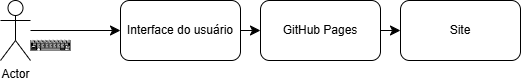
\includegraphics[width=0.8\textwidth]{solucao.drawio (1).png}
    \caption{Arquitetura da solução}
    \caption*{Fonte: Autoria própria.}
    \label{fig:Arquitetura da solução}
\end{figure}

A interface do usuário foi desenvolvida com tecnologias como HTML, CSS e JavaScript, proporcionando uma experiência visual responsiva, fluida e interativa. O site segue o modelo de página única (scroll único), em que todas as seções são acessadas verticalmente sem a necessidade de redirecionamentos.

O conteúdo do portfólio é exibido em seções organizadas, como “Sobre Mim”, “Estilo”, “Tecnologias” e “Certificados”. O sistema permite ainda a visualização de diplomas em formato de modal, além de conter redirecionamentos para redes sociais como GitHub e LinkedIn.

Para a hospedagem e disponibilização pública do projeto, foi utilizado o serviço do GitHub Pages, que permite o carregamento direto dos arquivos estáticos do repositório, garantindo fácil acesso ao site por meio de um link web. A arquitetura adotada garante simplicidade, manutenibilidade e acessibilidade para o cliente final.

\subsection{Requisitos Técnicos}

Nesta subseção, são apresentados os principais requisitos técnicos que nortearam o desenvolvimento do projeto, incluindo as ferramentas tecnológicas utilizadas, a organização da equipe e os métodos de acompanhamento do progresso.

\subsubsection{Ferramentas Tecnológicas}

O desenvolvimento do site foi realizado com base em tecnologias amplamente utilizadas no desenvolvimento web:

\begin{itemize}
\item \textbf{HTML5:} Utilizado para a estruturação semântica do conteúdo das páginas.
\item \textbf{CSS3:} Aplicado para a estilização e construção de um layout responsivo, garantindo boa experiência visual em diferentes dispositivos.
\item \textbf{GitHub Pages:} Plataforma utilizada para a hospedagem do site, possibilitando o acesso público ao projeto por meio de navegadores web.
\end{itemize}

\subsection{Modelagem dos processos}

A Figura \ref{fig:Modelagem dos processos} apresenta o fluxo de atividades realizadas durante o desenvolvimento do site portfólio, organizado em seis etapas sequenciais. O processo teve início com a coleta de informações junto ao cliente, na qual foram discutidas as necessidades, preferências estéticas e funcionalidades esperadas.

Na etapa seguinte, foi realizada a definição do layout e estilo visual, estabelecendo diretrizes como cores predominantes, tom da comunicação e escolha de ícones, com base nas preferências levantadas. Em seguida, procedeu-se com a estruturação do conteúdo, organizando as seções do portfólio e os textos informativos a serem exibidos.

Com o conteúdo e estilo definidos, passou-se à codificação do site em HTML e CSS, aplicando os conhecimentos técnicos para transformar o design em uma interface funcional. Após isso, foi feita a publicação do site na plataforma GitHub Pages, tornando-o acessível pela web.

Por fim, realizou-se a etapa de testes, ajustes e coleta de feedback, na qual o site foi avaliado para garantir a conformidade com os requisitos estabelecidos e permitir eventuais melhorias com base no retorno do cliente.

\begin{figure}[h!]
    \centering
    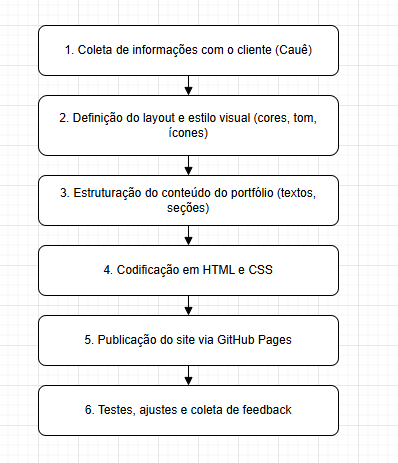
\includegraphics[width=0.8\textwidth]{fluxo_processos_desenvolvimento.png}
    \caption{Modelagem dos processos}
    \caption*{Fonte: Autoria própria.}
    \label{fig:Modelagem dos processos}
\end{figure}
    \chapter{Resultados}
\label{chap:result}

Este capítulo apresenta os principais resultados obtidos com o desenvolvimento do sistema, por meio de diagramas que ilustram as funcionalidades, a arquitetura e as interações entre os componentes da aplicação. Os diagramas foram elaborados com o objetivo de representar visualmente a estrutura e o funcionamento do sistema, facilitando a compreensão do seu comportamento e da sua modelagem. A seguir, são apresentados o diagrama de casos de uso, o diagrama de sequência e o diagrama de classes, cada um desempenhando um papel fundamental na documentação e análise do sistema.



\section{Diagrama de Casos de Uso}
\label{sec:casos}

O diagrama de casos de uso, apresentado na Figura \ref{fig:diagrama_uso}, representa as principais funcionalidades oferecidas pelo sistema e a forma como os atores interagem com ele. 

No sistema desenvolvido, existem dois atores principais: o \textbf{Desenvolvedor} e o \textbf{Usuário}. O Desenvolvedor tem permissão para \textit{Alterar Portfólio}, além de disponibilizar funcionalidades de visualização para o Usuário. Ambos os atores podem acessar os casos de uso de \textit{Visualizar perfil GitHub}, \textit{Visualizar perfil do LinkedIn} e \textit{Visualizar diploma}. 

Esses casos de uso demonstram as funcionalidades básicas voltadas à exibição de informações do portfólio do Desenvolvedor, com o objetivo de permitir que o Usuário visualize os conteúdos públicos disponibilizados.

\begin{figure}[h!]	
    \centering
    \caption{Diagrama de casos de uso}
    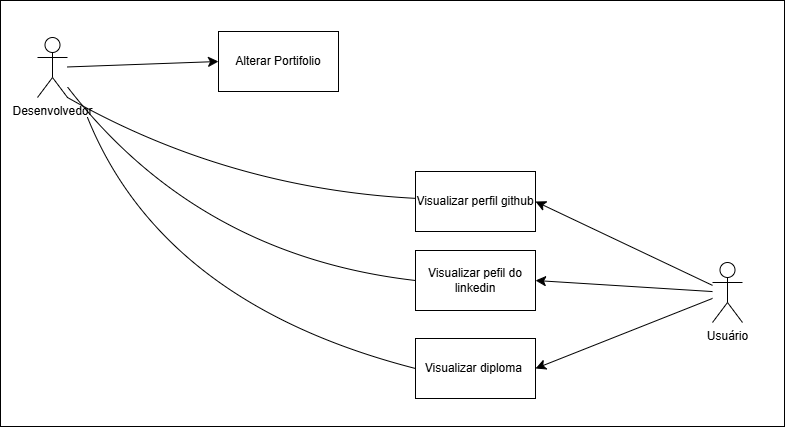
\includegraphics[width=0.8\textwidth]{Figures/diagrama_caso_uso.drawio.png}
    \caption*{Fonte: Autoria própria.}
    \label{fig:diagrama_uso}
\end{figure}

\clearpage
\section{Diagrama de Sequência}
\label{sec:sequencia}   

O diagrama de sequência, apresentado na Figura \ref{fig:diagrama_sequencia}, ilustra de forma detalhada o fluxo de interações entre os objetos do sistema ao longo do tempo para a realização de uma funcionalidade específica. Nele, é possível acompanhar a ordem cronológica das operações e a comunicação entre os componentes envolvidos, reforçando a dinâmica do comportamento do sistema.

Na sequência mostrada, o processo se inicia com a ação do \textbf{Usuário}, que, ao interagir com a interface (por exemplo, clicando em um elemento para visualizar um diploma ou acessar um link de rede social), desencadeia uma série de eventos. A \textbf{Interface de Usuário} registra esse evento e encaminha uma solicitação para o \textbf{Controlador} do sistema, que é responsável por processar a ação e gerenciar a lógica de negócio.

Após receber a solicitação, o Controlador realiza as seguintes etapas:
\begin{enumerate}
    \item Validação dos dados e verificação da integridade da requisição.
    \item Interação com a \textbf{Camada de Dados} para a recuperação das informações necessárias, como detalhes do diploma ou dados de perfis externos.
    \item Processamento dos dados recebidos e formatação da resposta para apresentação.
\end{enumerate}

Em seguida, o resultado desse processamento é devolvido ao usuário por meio da interface, seja na forma de uma exibição dinâmica (como a abertura de um modal com o diploma correspondente) ou do redirecionamento para uma página externa (como o perfil do LinkedIn ou GitHub).

Este diagrama evidencia a importância de uma comunicação clara e ordenada entre os componentes do sistema, assegurando que cada interação seja tratada de forma eficiente e que o fluxo de informações responda de maneira adequada às ações do usuário.

\begin{figure} [h!]	
    \centering
    \caption{Diagrama de sequencia}
    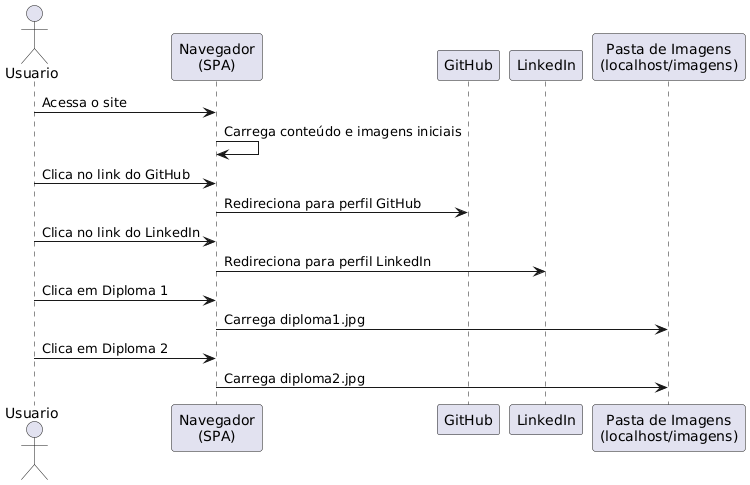
\includegraphics[width=0.8\textwidth]{Figures/diagrama_sequencia.png}
    \caption*{Fonte: Autoria própria.}
    \label{fig:diagrama_sequencia}
\end{figure}

\clearpage

\section{Diagrama de Classe}
\label{sec:classe}

O diagrama de classe, apresentado na Figura \ref{fig:diagrama_classe}, representa de forma estática a estrutura do sistema, evidenciando as classes que o compõem, seus atributos e os relacionamentos existentes entre elas. Essa representação facilita a compreensão da organização dos dados e das responsabilidades de cada entidade dentro do sistema.

No diagrama, a classe central é a Usuario, que possui atributos como fotoPerfil (do tipo FotoPerfil), foto (do tipo Foto), nome (do tipo string), além dos atributos diplomaUm e diplomaDois (ambos do tipo Diploma).

A classe Usuario está associada à classe Curriculo, indicando que um usuário pode possuir um currículo. A classe Curriculo contém atributos como usuario (do tipo Usuario), fotoUm e fotoDois (do tipo Foto), além de fotoGit e fotoLinkedin (ambos do tipo image).

Além disso, a classe Curriculo relaciona-se com a classe Projeto, permitindo que um currículo contenha múltiplos projetos. A classe Projeto possui atributos como curriculo (do tipo Curriculo) e mostrar\_projeto (também associado ao Curriculo).

Existem também classes auxiliares, como Diploma e FotoPerfil. A classe Diploma possui um atributo diploma (do tipo image), assim como a classe FotoPerfil que contém um atributo similar. Ambas são referenciadas pela classe Usuario, conforme indicado pelas linhas de associação no diagrama, sugerindo que um usuário possui ou utiliza instâncias dessas classes.

\begin{figure}[h!]
\centering
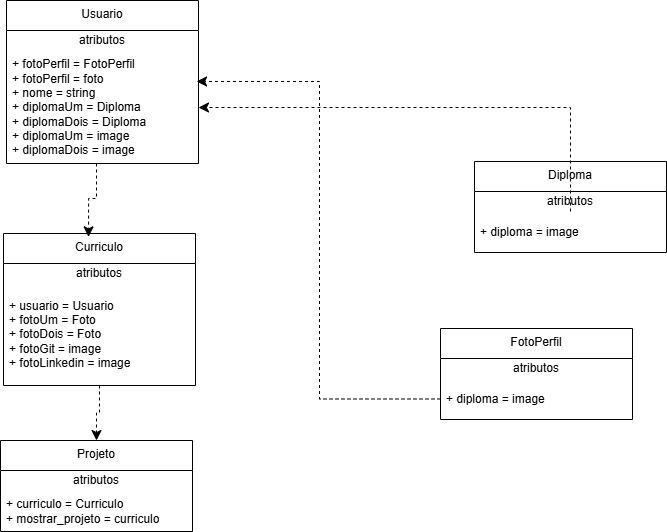
\includegraphics[width=0.8\textwidth]{Figures/diagrama_classe.drawio.png}
\caption{Diagrama de Classe do Sistema}
\caption*{Fonte: Autoria própria.}
\label{fig:diagrama_classe}
\end{figure}
    \chapter{Conclusão}
\label{chap:conc}

O desenvolvimento deste projeto proporcionou uma experiência prática completa em Análise e Projeto de Sistemas, permitindo à equipe aplicar conhecimentos teóricos em um cenário real com um cliente ativo. A criação do site portfólio envolveu etapas fundamentais como levantamento e análise de requisitos, modelagem de processos, elaboração de diagramas UML e desenvolvimento técnico com tecnologias amplamente utilizadas no mercado.

Ao longo do projeto, foi possível vivenciar as etapas do ciclo de vida de um sistema, desde a concepção inicial até a entrega final do produto. O uso de uma abordagem híbrida, mesclando o modelo Waterfall com práticas do Scrum, contribuiu para uma organização eficaz e para o acompanhamento contínuo das demandas do cliente.

Além dos aprendizados técnicos, o projeto também reforçou a importância da comunicação, da escuta ativa e do trabalho colaborativo. A entrega de um site funcional, visualmente coerente e que atende às expectativas do cliente demonstra não apenas a competência técnica da equipe, mas também seu compromisso com a qualidade e com o resultado final.

Assim, conclui-se que o projeto atingiu seus objetivos e proporcionou um desenvolvimento acadêmico e profissional significativo para todos os envolvidos, servindo como base sólida para futuros desafios na área de tecnologia.

\section{Considerações finais}
\label{sec:consid}

A execução deste projeto permitiu compreender, na prática, como a análise e o projeto de sistemas se conectam com as necessidades reais de um cliente. Mais do que aplicar ferramentas e técnicas, o processo exigiu sensibilidade para interpretar expectativas, adaptar soluções e tomar decisões com base em critérios técnicos e humanos.

Além do aprendizado técnico, o trabalho destacou o valor da empatia no relacionamento com o cliente, da responsabilidade com prazos e da colaboração entre os membros da equipe. Cada etapa, do levantamento de requisitos à entrega final, representou uma oportunidade de crescimento individual e coletivo.

Outro ponto importante foi a capacidade de adaptação: lidar com mudanças, revisar planos e ajustar entregas de acordo com o feedback recebido tornou-se um diferencial essencial para alcançar o resultado esperado.


    % include more chapters ...
%
% ----------------------------------------------------------------------------
% Include thesis appendices
    \begin{thesisappendices}
        \include{Appendices/diagmec}
        \include{Appendices/diagele}
        %\include{Appendices/logbook}
    \end{thesisappendices}
%
% ----------------------------------------------------------------------------

\renewcommand\bibname{Referências}
\addcontentsline{toc}{chapter}{Referências}
\bibliographystyle{abntex2-alf}
\bibliography{References/ref}


%
% ----------------------------------------------------------------------------
% Finishing him
    \include{Others/ultimafolha}
\end{document}
%
% -------------------------------------------------------------------------------
% Aqui termina a formatação para o documento.
% In God We Trust. All Other Bring Data. 
%
% -------------------------------------------------------------------------------